\section{Implementation}												
\label{sec:Implementation}
\lstset{numbers=left, breaklines=true,frame=shadowbox,
} 

\paragraph{}For the Android application, Android and Java were chosen as the primary programming languages due to the developer's familiarity with them. For the web interface, JSP was chosen as the background language. JavaScript and HTML were chosen to take care of the front-end and user interface. Ajax is also used to talk to the database. 

\subsection{Database Operations}
\label{subsec:DatabaseOperations}
\paragraph{}As what we mentioned in the design section, the Bmob online database was chosen for the database management system (DBMS) for both the Android application and the web interface. To use this database, we need an entity class to match each form. The entity class will extends BmobObject and the class name must be the same as the form name. As shown below:
\begin{lstlisting}[language=JAVA] 
public class Friend extends BmobObject {
    private String user;
    private String friend;
    public String getUser() {
        return user;
    }
    public void setUser(String user) {
        this.user = user;
    }
    public String getFriend() {
        return friend;
    }
    public void setFriend(String friend) {
        this.friend = friend;
    }
}
\end{lstlisting} 
\begin{figure}[htb]
\centering
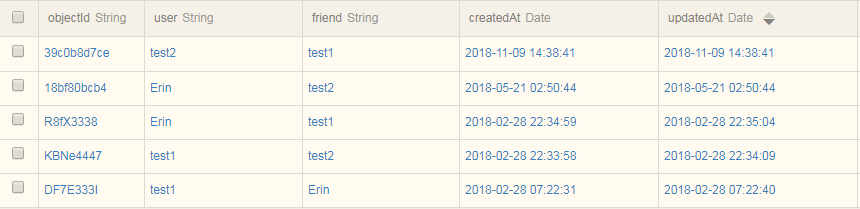
\includegraphics[width=.9\textwidth]{section04/assets/databaseOverview.png}
\caption[Short Caption]{\label{DatabseOverview}Form 'Friend'}
\end{figure}
\par Figure \ref{DatabseOverview} is the corresponding form in the database. The 'objectId', 'createdAt' and 'updatedAt' columns are generated by Bmob automatically. 
\par After we got the entity classes, we can begin to initialize. Three steps are needed for the initialization: 
\begin{enumerate}
\item[1)]Import SDK into your app level build.gradle file like this:
\begin{lstlisting}[language=JAVA] 
implementation 'cn.bmob.android:bmob-sdk:3.6.3'
\end{lstlisting} 
\item[2)] Configure AndroidManifest.xml file. This file is used to declare an application component and declare the permissions that the application needs. We will include this in later subsection \ref{subsubsec:GetSystemPermissions} Get System Permissions.
\item[3)] Initialize BmobSDK like the code shown below. The 'this' means the context and the 'ApplicationID' is defined when creating the project on Bmob website. The 'ApplicationID' is only accessible by the developer which maintains the security.
\begin{lstlisting}[language=JAVA] 
Bmob.initialize(this, "Your Application ID");
\end{lstlisting} 
\end{enumerate}
\par After initialization is finished. We can get access to the database like this:
\begin{lstlisting}[language=JAVA] 
BmobQuery<User> query = new BmobQuery<>();
query.addWhereEqualTo("username", username);
query.findObjects(new FindListener<User>() {
    @Override
    public void done(List<User> users, BmobException e) {
        if(e == null){
            System.out.println("EditProfile: query success");
            saveProfile(users.get(0),newPassword);
        }else{
            Log.i("bmob","failed:"+e.getMessage()+","+
            e.getErrorCode());
        }
    }
});
\end{lstlisting} 
\par All the data operations have a template which makes it easier to perform database operations.An inner class will be needed for each database operation. This piece of code shows how to retrieve data. Line 2 adds a constraint for the query which is the value of 'username' column equals the String username. The users in Line 5 will save the result if the query succeeded. If the error message, e, is null, then it means the query succeeded. 
\subsection{Image Processing Algorithms}
\paragraph{}This project addresses two central problems about image processing: transform the virtual gift to fit in user selected regions and find the correct region when user receive the gift. 

\subsubsection{Gift Transformation}
\paragraph{} Gift transformation is applies a perspective transformation of one image to another image. For perspective transformation, we need a 3x3 transformation matrix. Straight lines will remain straight even after the transformation. To find this transformation matrix, we need four points on the gift image which will be the four corners of the gift image and corresponding points on the background image. The corresponding points will be the four corners of the user selected region.  Among these four points, three of them should not be collinear. Then transformation matrix can be found by the function getPerspectiveTransform at Line 15. Then use the warpPerspective function at Line 16  to apply transformation with this 3x3 transformation matrix. The code below is the method used to apply transformation, drawable is the gift image, region is the background image, points contains the four corners user selected.
\begin{lstlisting}[language=JAVA] 
public Mat getThansform(Mat drawable, Mat region, int[] points) {
    Mat drawableCorner = new Mat(4, 1, CvType.CV_32FC2);
    Mat drawableTransformCorner = new Mat(4, 1, CvType.CV_32FC2);

    drawableCorner.put(0, 0, new double[]{0.0, 0.0});
    drawableCorner.put(1, 0, new double[]{drawable.cols(), 0.0});
    drawableCorner.put(2, 0, new double[]{drawable.cols(), drawable.rows()});
    drawableCorner.put(3, 0, new double[]{0.0, drawable.rows()});

    drawableTransformCorner.put(0, 0, new double[]{points[0], points[1]});
    drawableTransformCorner.put(1, 0, new double[]{points[2], points[3]});
    drawableTransformCorner.put(2, 0, new double[]{points[4], points[5]});
    drawableTransformCorner.put(3, 0, new double[]{points[6], points[7]});

    Mat perspectiveTransform = Imgproc.getPerspectiveTransform(drawableCorner, drawableTransformCorner);
    Imgproc.warpPerspective(drawable,region,perspectiveTransform, region.size(), Imgproc.INTER_LINEAR,
    Core.BORDER_TRANSPARENT, new Scalar(0, 0, 0, 0));

    return region;
}
\end{lstlisting} 
\subsubsection{Region Recognition}
\paragraph{}Image recognition is more complex, we used 'Features2D' and 'Homography' in OpenCv to find a known object in a real time camera capture frame. The steps and corresponding code are listed below:
\begin{enumerate}
\item[1)] Detect the keypoints using AKAZE Detector. This piece of code put the ProcessedCamera image keypoints in cameraKeypoints.
\begin{lstlisting}[language=JAVA] 
FeatureDetector featureDetector = FeatureDetector.create(FeatureDetector.AKAZE);
MatOfKeyPoint cameraKeypoints = new MatOfKeyPoint();
Imgproc.cvtColor(processedCamera, processedCamera, Imgproc.COLOR_RGBA2RGB);
featureDetector.detect(processedCamera, cameraKeypoints);
\end{lstlisting} 
\item[2)] Calculate descriptors (feature vectors). We get cameraDescriptor for processedCamera here.
\begin{lstlisting}[language=JAVA] 
DescriptorExtractor extractor = DescriptorExtractor.create(DescriptorExtractor.AKAZE);
Mat cameraDescriptor = new Mat();
extractor.compute(processedCamera, cameraKeypoints, cameraDescriptor);
\end{lstlisting} 
\item[3)] Matching descriptor vectors using 'BRUTEFORCE\_HAMMING' matcher and only save 'good' matches, the smaller distance means better match and here we only get the first half matches. 
\begin{lstlisting}[language=JAVA] 
MatOfDMatch matches = new MatOfDMatch();
DescriptorMatcher matcher = DescriptorMatcher.create(DescriptorMatcher.BRUTEFORCE_HAMMING);
matcher.match(cameraDescriptor, giftDescriptor, matches);
            
List<DMatch> bestMatchesList = mats.stream().filter( m -> (m.distance - MIN_DIST) < .5 * range)
                    .collect(Collectors.toList());
\end{lstlisting} 
\item[4)] Get the keypoints from the 'good' matches.
\begin{lstlisting}[language=JAVA] 
 for(int i=0; i<bestMatchesList.size(); i++){
    objectPoints.addLast(templateKeyPointList.get(bestMatchesList.get(i).trainIdx).pt);
    scenePoints.addLast(originalKeyPointList.get(bestMatchesList.get(i).queryIdx).pt);
}
\end{lstlisting} 
\item[5)] Get the four corners from the selected region. Here we use a Mat with one column four rows to save the points. points is an array of String with user selected region information.
\begin{lstlisting}[language=JAVA] 
Mat templateCorners = new Mat(4, 1, CvType.CV_32FC2);
templateCorners.put(0, 0, new double[]{points[0], points[1]});
templateCorners.put(1, 0, new double[]{points[2], points[3]});
templateCorners.put(2, 0, new double[]{points[4], points[5]});
templateCorners.put(3, 0, new double[]{points[6], points[7]});
\end{lstlisting} 
\item[6)] Use perspectiveTransform method to localize the object. The four detected corners of region is now saved in templateTransformResult.
\begin{lstlisting}[language=JAVA] 
Core.perspectiveTransform(templateCorners, templateTransformResult, homography);
\end{lstlisting} 
\end{enumerate}

\subsection{Android Application}
\subsubsection{Usage of Adapter}
\paragraph{}
An Adapter object acts as a bridge between an AdapterView (e.g. ListView, Spinner, and GridView) and the underlying data for that view. The Adapter provides access to the data items. The Adapter is also responsible for making a View for each item in the data set. For this project, ListView is used to show friends list and gifts list shown in Figure \ref{FriendsListUI} Friends List page and Figure \ref{GiftsListUI} Gifts List page. GridView is used to show the gifts selection after users choose a region. Figure \ref{AdapterOverview} shows a overview of adapter.
\begin{figure}[htb]
\centering
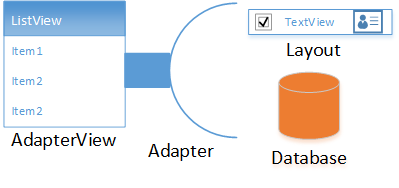
\includegraphics[width=.7\textwidth]{section04/assets/AdapterOverview.png}
\caption[Short Caption]{\label{AdapterOverview}Overview of Adapter}
\end{figure}

\subsubsection{Get system permissions}
\label{subsubsec:GetSystemPermissions}
\paragraph{} As mentioned in Section \ref{subsec:DatabaseOperations} Database Operations, we need to configure AndroidManifest.xml file. This file is used to declare an application component and declare the permissions that the application needs. As shown below, Line 1 is used to get the internet permission, Line 2 is used to get the external storage permission, and Line 3 is needed to create BmobInstallation. Line 4 is to acquire the system camera permission, we will need this when users send a gift and when users find a gift. Line 5 is used to get user locations. Android offers two location permissions: ACCESS\_COARSE\_LOCATION and ACCESS\_FINE\_LOCATION. The permission you choose determines the accuracy of the location returned by the API. If you specify ACCESS\_COARSE\_LOCATION, the API returns a location with an accuracy approximately equivalent to a city block. However, 'ACCESS\_FINE\_LOCATION' allows an app to access precise location.
\begin{lstlisting}[language=JAVA] 
<uses-permission android:name="android.permission.INTERNET" />
<uses-permission android:name="android.permission.WRITE_EXTERNAL_STORAGE" />
<uses-permission android:name="android.permission.READ_PHONE_STATE" />
<uses-permission android:name="android.permission.CAMERA" />
<uses-permission android:name="android.permission.ACCESS_FINE_LOCATION" />
\end{lstlisting} 
\par The other usage of this file is define an Activity, the code below shows an example. In this example, the Acitivity is named 'SignInActivity' and it is a launcher for this application.
\begin{lstlisting}[language=JAVA] 
<activity
    android:name=".SignInActivity"
    android:label="@string/title_activity_sign_in">
    <intent-filter>
        <action android:name="android.intent.action.MAIN" />
        <category android:name="android.intent.category.LAUNCHER" />
    </intent-filter>
</activity>
\end{lstlisting} 

\subsubsection{Call Camera}
\paragraph{} The Camera is another important part in this project. There are two functions which use camera: 'Send a gift' and 'Receive a gift'.
Other than get user permissions mentioned in section \ref{subsubsec:GetSystemPermissions} Get System Permissions, this chunk of code shows an example of calling the system camera. Line 2 to Line 8 creates a file in storage. Line 12 called the system camera and Line 20 saved the picture into the system album. In Line 15 we have a check for sdk version, that is because if the targetSdkVersion >= 24, then we have to use FileProvider class to give access to the particular file or folder to make them accessible for other apps. FileProvider is a special subclass of ContentProvider that facilitates secure sharing of files associated with an app by creating a 'content:// Uri' for a file instead of a 'file:/// Uri'. A content URI allows you to grant reading and writing access using temporary access permissions. 
\begin{lstlisting}[language=JAVA] 
private void sendMessage() {
    File mediaStorageDir = new File(Environment.getExternalStoragePublicDirectory(
            Environment.DIRECTORY_PICTURES), "giftbox");
    if (!mediaStorageDir.exists()) {
        if (!mediaStorageDir.mkdirs()) {
            Log.d("MyCameraApp", "failed to create directory");
        }
    }
    String timeStamp = new SimpleDateFormat("yyyyMMdd_HHmmss").format(new Date());
    image = new File(mediaStorageDir.getPath() + File.separator +
            "IMG_" + timeStamp + ".jpg");
    Intent intent = new Intent(MediaStore.ACTION_IMAGE_CAPTURE);
    intent.addCategory(Intent.CATEGORY_DEFAULT);
    Uri uri;
    if (Build.VERSION.SDK_INT >= Build.VERSION_CODES.N) {
        uri = FileProvider.getUriForFile(thisContext, BuildConfig.APPLICATION_ID+".fileprovider", image);//BuildConfig.APPLICATION_ID + ".fileProvider"
    } else {
        uri = Uri.fromFile(image);
    }
    intent.putExtra(MediaStore.EXTRA_OUTPUT, uri);
    startActivityForResult(intent, 0);
}
\end{lstlisting} 
\par After this we will be able to get the result in onActivityResult method.